%%%%%%%%%%%%%%%%%%%%%%%%%%%%%%%%%%%%%%%%%%%%%%%%%%%%%%%%%%%%
\chapter{Experimental Evaluation}
\label{chap:eval}
In this chapter, we present different methods of evaluation and analysis for entity embeddings and the faceted models. In Section~\ref{sec:eval_embeddings}, most common methods for evaluation of word embeddings are discussed and the ones chosen for this study are presented. Section ~\ref{sec:data} explains the dataset used for training the embeddings, the preprocessing and graph extraction.Evaluation setup and parameter tuning for the models is discussed in in Section~\ref{sec:setup}. Evaluation results for the common tasks are shown in Section~\ref{sec:eval_results}, where the results for the entity embeddings and faceted models are discussed separately in Subsections~\ref{subsec:eval_entity} and \ref{subsec:eval_faceted} respectively. Finally, in Section~\ref{sec:eval_experimental} contains the experimental exploration and visualization of the embeddings neighbourhood. 
\section{Evaluation of Word Embeddings}\label{sec:eval_embeddings}
In general, the evaluation of word embeddings falls into two major categories: the extrinsic and intrinsic evaluation. In an extrinsic evaluation trained embeddings are used as input of some downstream task and the performance is measured by a metric specific to that task, such as part-of-speech tagging, named-entity recognition and event summarization. However, since evaluations are task-specific, an embedding that works well for one task may fail for another. Intrinsic evaluations directly test for syntactic or semantic relationships between words. These tasks analyze how well the embeddings capture certain syntactic or semantic relations between a set of query and target words, referred to as \textit{query inventory}~\brackettext{\cite{DBLP:conf/emnlp/SchnabelLMJ15}}. Intrinsic tasks are easier and faster to test and provide a quick understanding of the system. The problem with such tests is that the notion of semantics is not universal~\brackettext{\cite{DBLP:journals/corr/abs-1801-09536}}. Some datasets reflect semantic relatedness and some semantic similarity, while very similar they measure quite different attributes. Two words are considered semantically similar, that are synonymy and can be substituted for each other in context. For instance, \emph{``rose"} and \emph{``flower"}. Semantic relatedness, however, is a broader concept. Words with any functional associations, like belongin to the same semantic field, are considered semantically related, e.g., \emph{``rose"} and \emph{``thorn"} ~\brackettext{\cite{DBLP:conf/nodalida/Kolb09}}. It is not obvious, if the word embedding should favour relatedness over similarity or visa versa. Furthermore, a high accuracy on these tasks does not necessarily mean that the model will perform well on real tasks unless some correlation between them is established. Thus, testing the model on an intrinsic task at first and an extrinsic task in final steps can provide a better overview of the model performance. Since there are no entity-centric extrinsic evaluation tasks in the literature and few intrinsic data sets include entities, we focus on the performance in term-based intrinsic tasks. We create some of our own datasets to incorporate the entities, but it is important to emphasize that the true potential of these entity-based models can only be truely investigated in the presence of suitable evaluation datasets.Following the approach by~\brackettext{\cite{DBLP:conf/emnlp/SchnabelLMJ15}}, we use three kinds of intrinsic evaluations.
 \subsubsection{Relatedness}
This task is based on datasets containing relatedness or similarity scores for pairs of words annotated by humans; the cosine similarity or Euclidean distance between the embeddings for two words should have high correlation (Spearman or Pearson) with human similarity or relatedness scores. We choose seven datasets containing both relatedness and similarity scores. 
\begin{enumerate}
 \item \emph{Similarity353:} $203$ instances of similar word pairs from WordSim353~\brackettext{\cite{DBLP:conf/naacl/AgirreAHKPS09}} classified as synonyms, antonyms, or identical, and unrelated pairs (pairs with average similarity less than or equal to $5$). Scores scale from 0 (totally unrelated words) to 10 (very much related or identical words).~\brackettext{\cite{DBLP:conf/naacl/AgirreAHKPS09}}.
 \item \emph{Relatedness353:} $252$ instances of word pairs from WordSim353~\brackettext{\cite{DBLP:conf/naacl/AgirreAHKPS09}} that are not similar but still considered related by humans, with an average similarity greater than $5$, and unrelated pairs~\brackettext{\cite{DBLP:conf/naacl/AgirreAHKPS09}}.
 \item \emph{MEN:} $3,000$ word pairs with human-assigned similarity judgements, which instead of an absolute score is based on comparative judgments on two pair exemplars at a time. Each person was given a binary choice of \emph{``right''} or \emph{``wrong''} and in total each pair was compared $50$ times, thus obtaining a final score on a $50$-point scale~\brackettext{\cite{DBLP:journals/jair/BruniTB14}}.
 \item \emph{RG65:} $65$ pairs with annotated similarity scaling from $0$ to $4$, where the similarity between two words is measured by the similarity of meaning and the
amount of overlap for each definition of context. ~\brackettext{\cite{DBLP:journals/cacm/RubensteinG65}}.
 \item \emph{RareWord:} $2,034$ rare word pairs with human similarity scores~\brackettext{\cite{DBLP:conf/conll/LuongSM13}}.
 \item \emph{SimLex-999:} $999$ pairs of human-labeled examples of semantic relatedness~\brackettext{\cite{DBLP:journals/corr/HillRK14}}.
 \item \emph{MTurk:} $7,714$ words pairs with semantic relatedness scores from
$0$ to $5$~\brackettext{\cite{Radinsky:2011:WTC:1963405.1963455}}.
\end{enumerate}

\subsubsection{Analogy}
This task was popularized by the word2vec paper~\cite{DBLP:journals/corr/abs-1301-3781}, where the goal is to find a term $x$ for a given term $y$, such that  $x : y$ best resembles a sample relationship $a : b$. In other words, given the triple $(a,b,x)$, the aim is to find the target word $y$ correctly. To find the target word we do the following:  
\begin{itemize}
    \item Compute $w_a-w_b=w_{a-b}$, where $w_a$ and $w_b$ are the embeddings for word $a$ and $b$. 
    \item  Compute the mean vector $w_{mean}=w_{a-b}+w_x$.
    \item  Find the nearest neighbour to $w_{mean}$ (the one with the highest cosine similarity) if it is $w_y$, the analogy was found correctly.
  \end{itemize}
  \noindent
For entity embeddings, where the type of the embedding is known, we can also consider an easier, type-specific variation of this task, which only considers neighbours that match a given entity class. In the type-specific variation we only consider candidates that have the same entity type as the words in the triple $(a,b,x)$, thus making the task easier. 
\subsubsection{Categorization}
When projecting the word embedding in a 2 or 3-dimensional space, iwe expected that the similar words form meaningful clusters. The embedding can be projected using \emph{t-SNE}~\cite{SCHOL:journals/jmlr/Maaten} or \emph{Principle Component Analysis (PCA)}. Vectors of all words are either viualized for exploratory analysis or clustered using a clustering algorithm of choice and the purity of the returned clusters is computed as a metric for this task~\brackettext{\cite{DBLP:books/daglib/0021593}}. 

\section{Training Data}\label{sec:data}

The models were trained on a subset of news articles from the English speaking outlet, the New York Times. The collection contains data for six months from June $1, 2016$ to November $30$, $2016$. There were total of $5,439$ article and $5,427,383$ sentences used.The news articles were used to create the LOAD network, which itself is a collection of nodes annotated by type and weighted edges that are used directly to generate the weighted adjacency matrices. The generated LOAD network contains $93,390$ nodes and $9,584,191$ edges. The number of nodes in each type is different, with the terms being the most frequent and dates the least frequent type. There exists $2,442$ date entities, $4,659$ location, $10,537$ actors, $3,789$ organisations and $71,963$ terms in total. For GloVe and word2vec a textual corpus was created by replacing the raw text form with the given LOAD node identifiers, to generate comparable results. Because the normal text contains stop-words and unwanted characters, terms were filtered to only necessary parts of speech tags for the model generation. The final corpus contains $4,468,993$ tokens, where each token is the node identifier of the respective entity or term in the LOAD network. 
 
 \section{Parameter Tuning } \label{sec:setup}

For the ease of use, the following naming convention is used to distinguish different models: Name of the Method\_\{additional parameters\}, where additional parameters show the different hyper-parameters or additional changes to the original model. 
\begin{itemize}
\item  \textbf{F:} Focal addition, which means rather than the pure context embedding for each type the respective focal embeddings were added back to the model with selective addition. 
\item \textbf{W:} Short for weighted. In this case, the weighing function was used to cap the importance of highly frequent words with large weights. 
\item \textbf{C$\{ number \}$:} Shows the value for $x_{max}$ or co-occurrence cap in the model, which is the maximum weight in the weighing function. 
\item \textbf{S$\{ number \}$:} Shows the scaling factor of or $\alpha$ in the weighing function. This number is always between $0$ and $1$. For example $S5$ indicates $\alpha=0.5$ and $S75 $ shows $\alpha=0.75$. 
\item \textbf{L:} Shorten for $log+1$.we tested the model with the addition of $1$ to the log of weights, to help distinguish between weights of $0$ and $1$. 

\item \textbf{Uni:} Indicates that the model was trained using the unified cost function. If not present, the separate cost function was used. 
\end{itemize}

The weighing function was used in the model to boost the weak connections and stop the model from giving more weights to the edges with large weights. In case of the hyper-parameters, $\alpha$ and $x_{max}$ we did additional tuning. For $\alpha=[1,0.75,0.5,0.25,0]$ and for $x_{max}=[10,100,1000,10000]$ were experimented. Setting the $x_{max}$ to a number larger numbers, such as, $10000$ produced the best result. In case of a scaling factor, the suggested value by the author ($\frac{3}{4}$) led to the best result. 
Unified cost and focal addition were treated as a binary parameter (either present during training or removed). Instead of a typical grid search, we chose a coarse-to-fine method, where instead of checking all the possible combinations, we randomly sampled some parameters and focused on the areas, where better models were trained. For example, focal addition proved to be beneficial in most cases, therefore, most of the models contain this attribute.\\

\noindent
All the models were trained for $200$ epochs with a learning rate of $0.05$ and a batch size of $256$. In addition, as a preprocessing step, all the edges for all the entities which occur less than five times in the corpus were removed from the input data. \\
The facetted embedding, with or without unified cost, produced almost identical results, but when trained with separate costs, the training phase is faster. For that reason, only one instance of the facetted model with a unified cost is present in the results. \\
\noindent
All the created models were compared against two well-known models: GloVe and word2vec. Both of which were trained for $200$ epochs on a textual corpus of all the articles, with a learning rate of $\alpha=0.05$ and $\alpha=0.025$, respectively. Since the GloVe model also works on the whole corpus statistic, the words with the frequency less than five were removed from the model as a preprocessing step. For word2vec, on the other hand, such a property does not exist. 

\begin{figure}
\centering
\subcaptionbox{\label{sfig:full_wordsim}}{
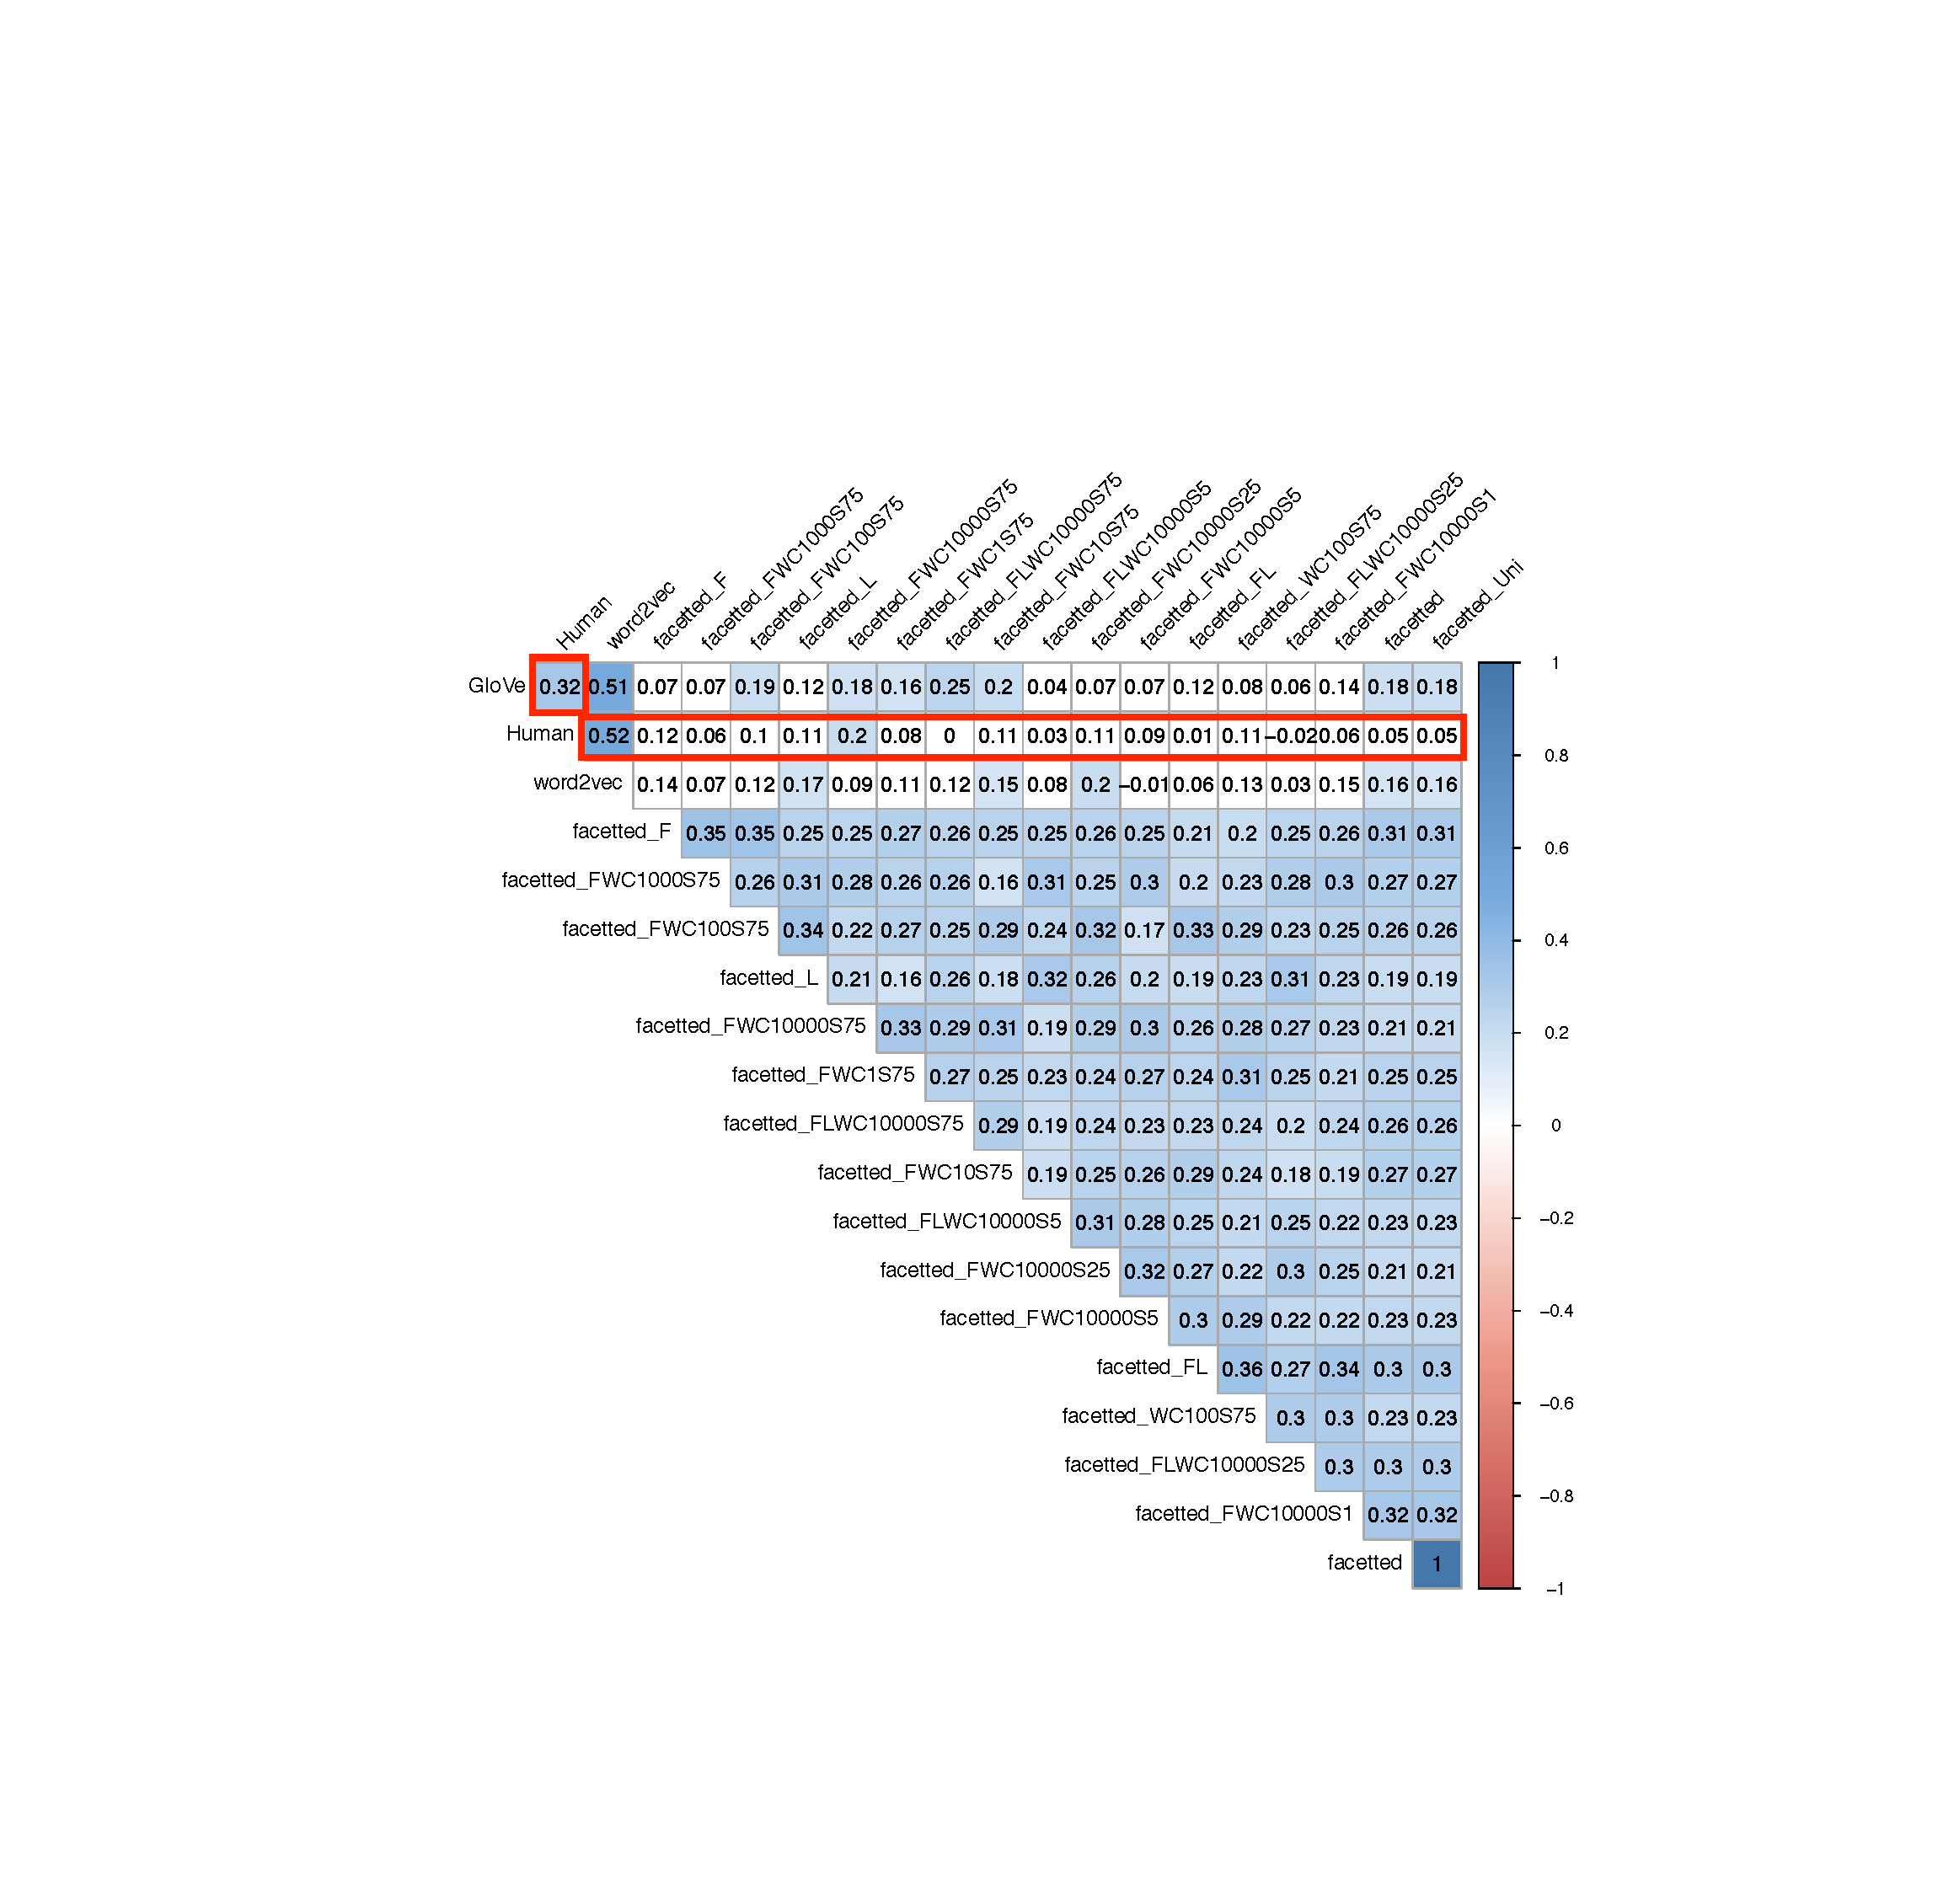
\includegraphics[width=0.75\linewidth , height=0.65\linewidth]{images/Corr_plot_full_sim.pdf}}
\subcaptionbox{\label{sfig:part_wordsim}}{
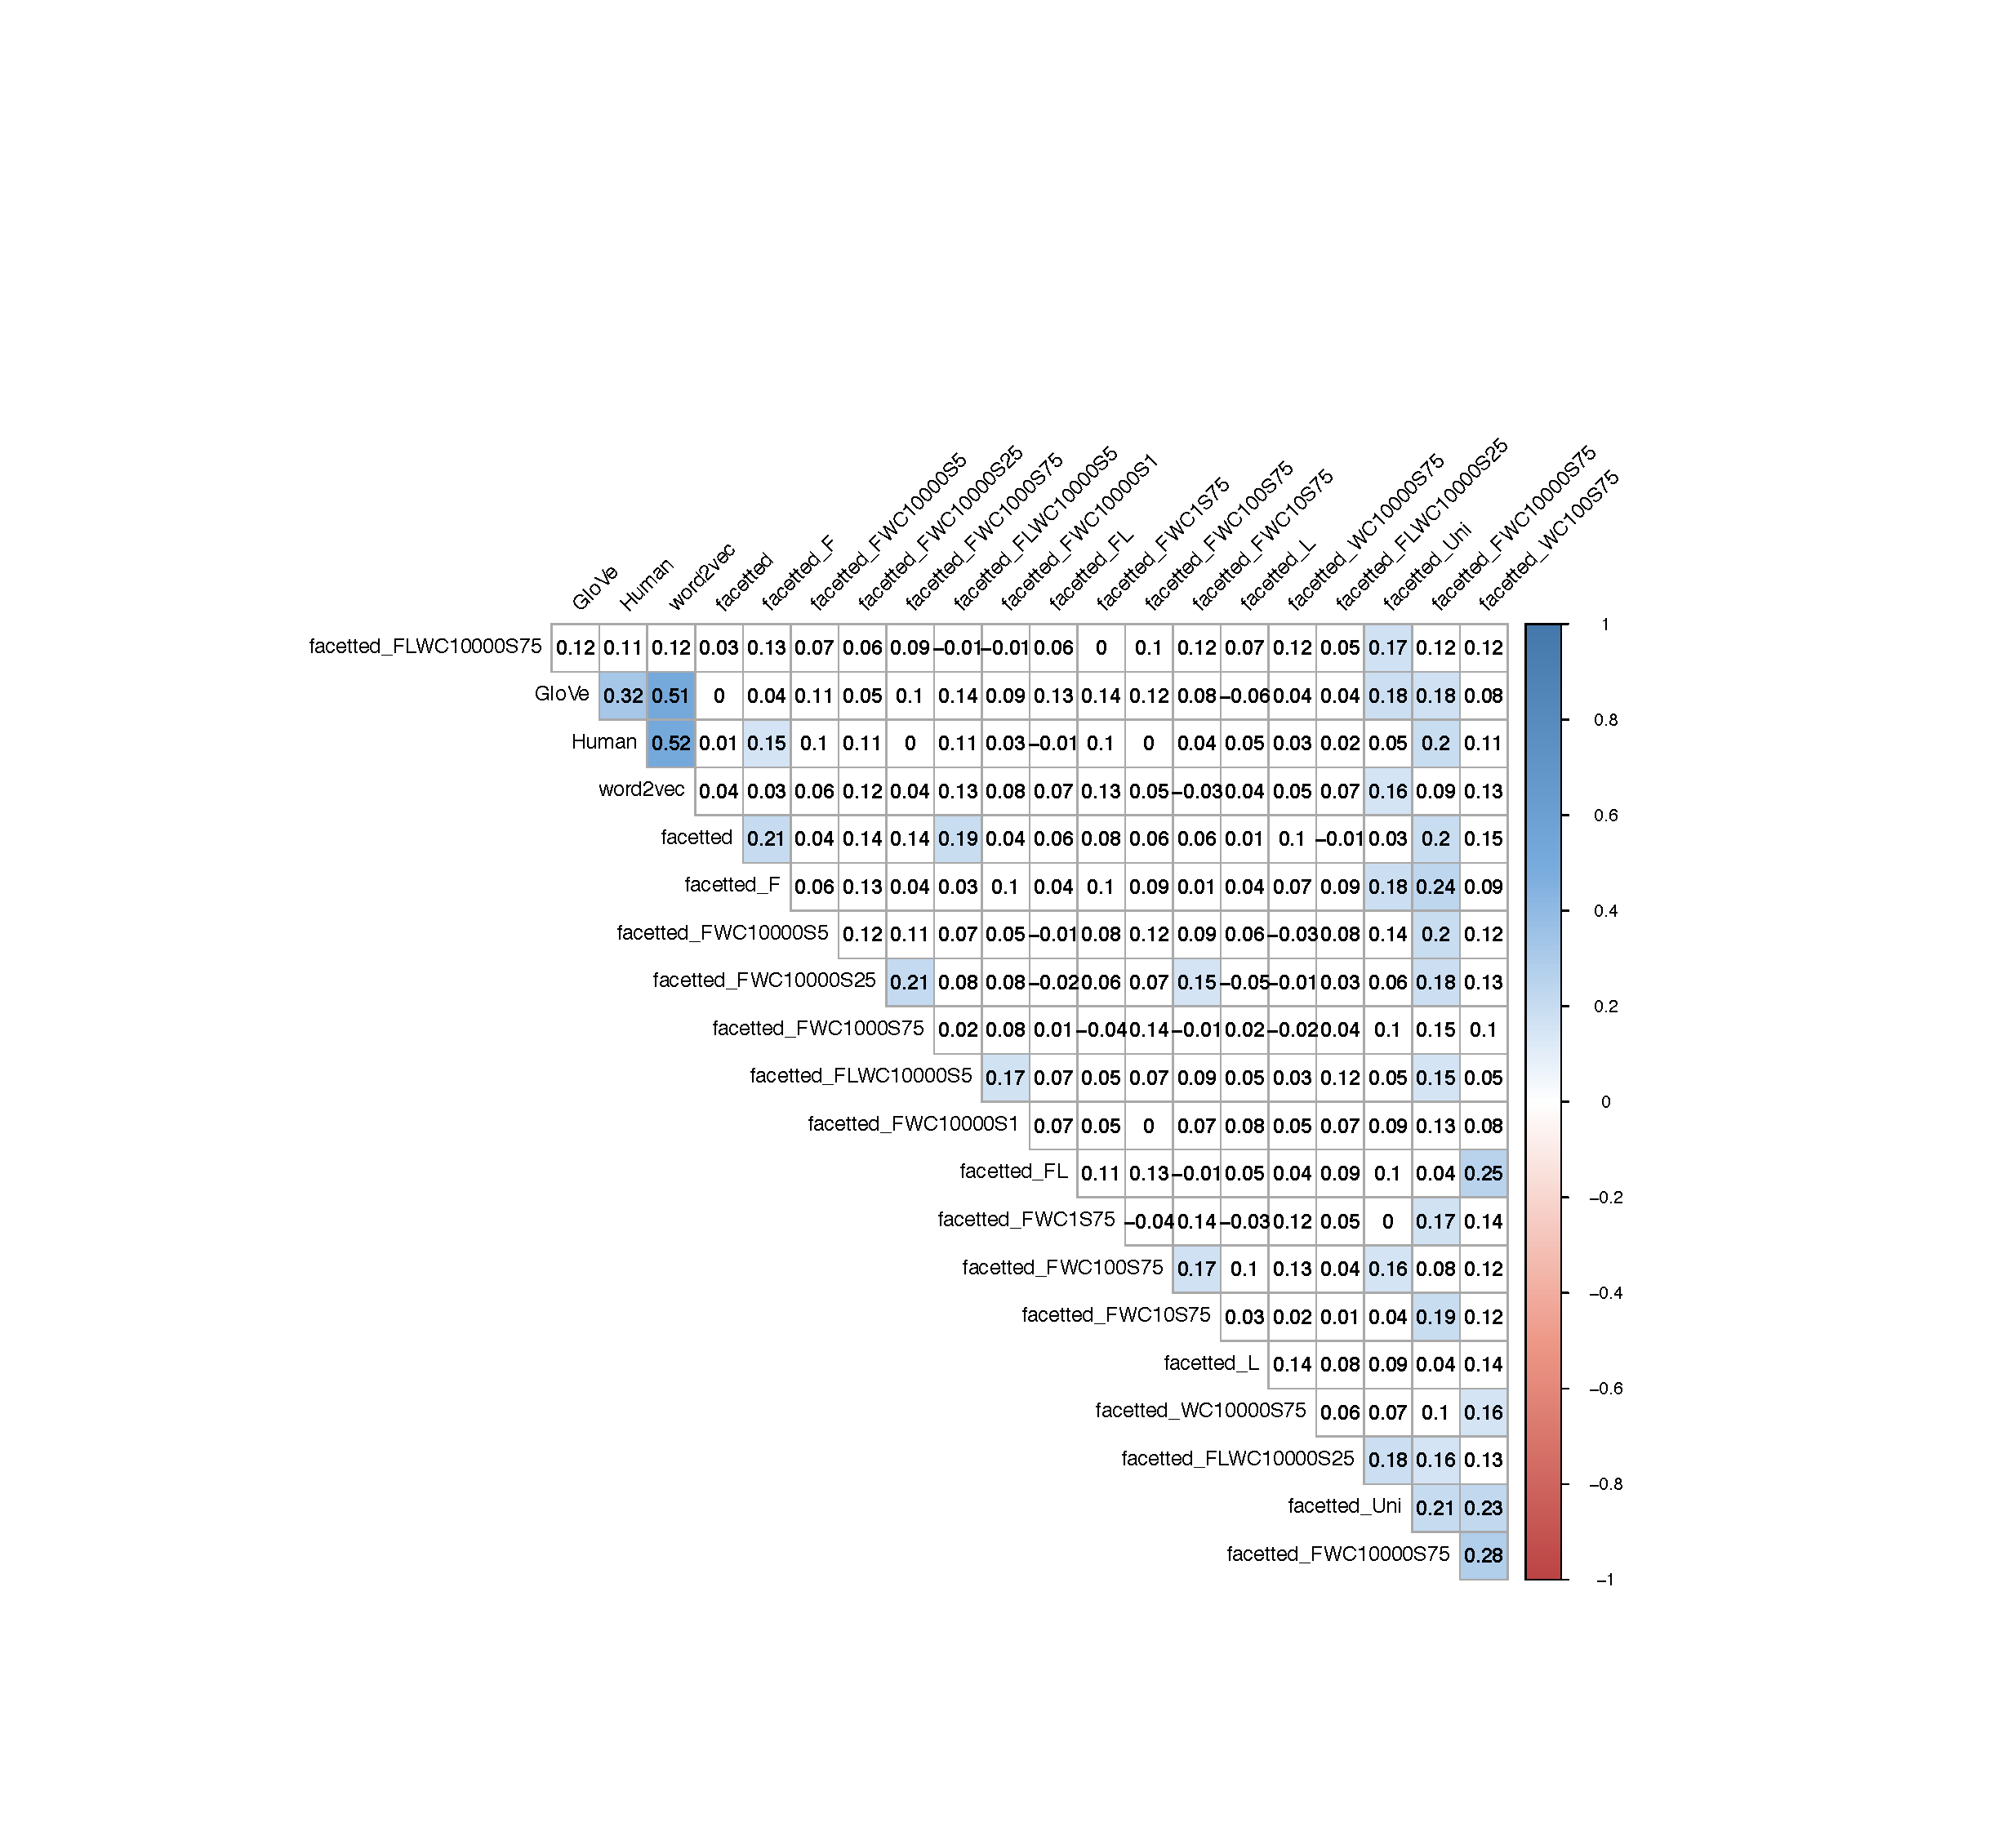
\includegraphics[width=0.80\linewidth , height=0.65\linewidth]{images/wordsim_partial.pdf}}

\caption{Correlation plot of the relatedness scores on wordsim353 using the~\subref{sfig:full_wordsim} full vectors and ~\subref{sfig:part_wordsim} using type-specific vectors. Red highlights show the correlation with the human annotations.}
\label{fig:wordsim_cor}
\end{figure}


\section{Evaluation Results}\label{sec:eval_results}
\subsection{Evaluation of entity embeddings}\label{subsec:eval_entity}
\subsection{Evaluation of faceted embeddings}\label{subsec:eval_faceted}

\section{Experimental Exploration}\label{sec:eval_experimental}
\subsection{Analysis of entity embeddings}\label{subsec:exp_entity}
\subsection{Analysis of faceted embeddings}\label{subsec:exp_faceted}

\section{Word Relatedness}\label{sec:relatedness}

Two dataset were chosen for comparing the relatedness scores, namely: \emph{wordsim353}~\cite{DBLP:conf/www/FinkelsteinGMRSWR01} and \emph{MEN}~\cite{DBLP:journals/jair/BruniTB14}. Wordsim353 contains $353$ sets of English word pairs along with human-assigned similarity judgments on a scale from $0$ (totally unrelated words) to $10$ (very much related or identical words). After filtering the set to match the entities available in our model $294$ word pairs were left. MEN dataset consists of
$3,000$ word pairs, which instead of an absolute score is based on comparative judgments on two pair exemplars at a time. Each person was given a binary choice of ``right'' or ``wrong'' and in total each pair was compared $50$ times, thus obtaining a final score on a $50$-point scale. After filtering, $2,225$ pairs remained in the dataset.\\
Since wordsim353 was the smaller set and could be evaluated quickly, this dataset was used as a semi-development set, where the models with different hyper-parameters were compared and only the most successful ones were later tested on the MEN dataset as well. \\
Correlation plots for the partial and full similarities can be seen in Figures~\ref{sfig:full_wordsim} and~\ref{sfig:part_wordsim}. The most significant rows and columns are marked in red, which illustrates the correlation between the human annotators and the cosine similarity of the word vectors. Correlations were computed using \emph{Pearson} method and any cell with correlation with p-value bigger than $0.01$ is colored in blue.
Some important observations from the correlation plot can be listed as follows:\\
\begin{figure}[hb]
\centering
\subcaptionbox{\label{sfig:scaling_f}}{
\resizebox{0.45\textwidth}{0.30\textwidth}{      

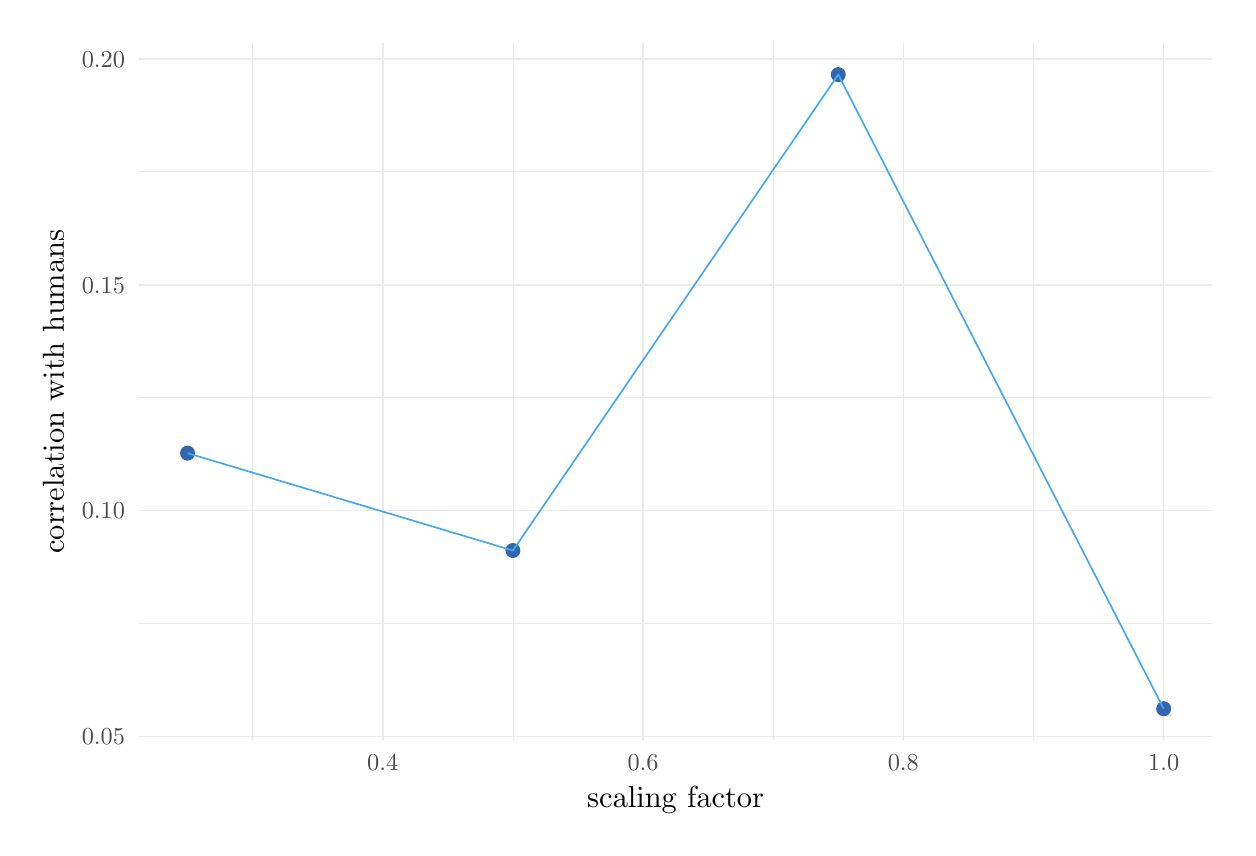
\begin{tikzpicture}[x=1pt,y=1pt]
\definecolor{fillColor}{RGB}{255,255,255}
\path[use as bounding box,fill=fillColor,fill opacity=0.00] (0,0) rectangle (433.62,289.08);
\begin{scope}
\path[clip] ( 40.14, 31.53) rectangle (428.12,283.58);
\definecolor{drawColor}{gray}{0.92}

\path[draw=drawColor,line width= 0.3pt,line join=round] ( 40.14, 73.78) --
	(428.12, 73.78);

\path[draw=drawColor,line width= 0.3pt,line join=round] ( 40.14,155.37) --
	(428.12,155.37);

\path[draw=drawColor,line width= 0.3pt,line join=round] ( 40.14,236.97) --
	(428.12,236.97);

\path[draw=drawColor,line width= 0.3pt,line join=round] ( 81.29, 31.53) --
	( 81.29,283.58);

\path[draw=drawColor,line width= 0.3pt,line join=round] (175.34, 31.53) --
	(175.34,283.58);

\path[draw=drawColor,line width= 0.3pt,line join=round] (269.40, 31.53) --
	(269.40,283.58);

\path[draw=drawColor,line width= 0.3pt,line join=round] (363.46, 31.53) --
	(363.46,283.58);

\path[draw=drawColor,line width= 0.6pt,line join=round] ( 40.14, 32.98) --
	(428.12, 32.98);

\path[draw=drawColor,line width= 0.6pt,line join=round] ( 40.14,114.58) --
	(428.12,114.58);

\path[draw=drawColor,line width= 0.6pt,line join=round] ( 40.14,196.17) --
	(428.12,196.17);

\path[draw=drawColor,line width= 0.6pt,line join=round] ( 40.14,277.76) --
	(428.12,277.76);

\path[draw=drawColor,line width= 0.6pt,line join=round] (128.32, 31.53) --
	(128.32,283.58);

\path[draw=drawColor,line width= 0.6pt,line join=round] (222.37, 31.53) --
	(222.37,283.58);

\path[draw=drawColor,line width= 0.6pt,line join=round] (316.43, 31.53) --
	(316.43,283.58);

\path[draw=drawColor,line width= 0.6pt,line join=round] (410.48, 31.53) --
	(410.48,283.58);
\definecolor{drawColor}{RGB}{50,103,173}
\definecolor{fillColor}{RGB}{50,103,173}

\path[draw=drawColor,line width= 0.4pt,line join=round,line cap=round,fill=fillColor] ( 57.77,135.33) circle (  2.50);

\path[draw=drawColor,line width= 0.4pt,line join=round,line cap=round,fill=fillColor] (175.34,100.15) circle (  2.50);

\path[draw=drawColor,line width= 0.4pt,line join=round,line cap=round,fill=fillColor] (292.91,272.12) circle (  2.50);

\path[draw=drawColor,line width= 0.4pt,line join=round,line cap=round,fill=fillColor] (410.48, 42.99) circle (  2.50);
\definecolor{drawColor}{RGB}{66,167,244}

\path[draw=drawColor,line width= 0.6pt,line join=round] ( 57.77,135.33) --
	(175.34,100.15) --
	(292.91,272.12) --
	(410.48, 42.99);
\end{scope}
\begin{scope}
\path[clip] (  0.00,  0.00) rectangle (433.62,289.08);
\definecolor{drawColor}{gray}{0.30}

\node[text=drawColor,anchor=base east,inner sep=0pt, outer sep=0pt, scale=  0.88] at ( 35.19, 29.95) {0.05};

\node[text=drawColor,anchor=base east,inner sep=0pt, outer sep=0pt, scale=  0.88] at ( 35.19,111.55) {0.10};

\node[text=drawColor,anchor=base east,inner sep=0pt, outer sep=0pt, scale=  0.88] at ( 35.19,193.14) {0.15};

\node[text=drawColor,anchor=base east,inner sep=0pt, outer sep=0pt, scale=  0.88] at ( 35.19,274.73) {0.20};
\end{scope}
\begin{scope}
\path[clip] (  0.00,  0.00) rectangle (433.62,289.08);
\definecolor{drawColor}{gray}{0.30}

\node[text=drawColor,anchor=base,inner sep=0pt, outer sep=0pt, scale=  0.88] at (128.32, 20.52) {0.4};

\node[text=drawColor,anchor=base,inner sep=0pt, outer sep=0pt, scale=  0.88] at (222.37, 20.52) {0.6};

\node[text=drawColor,anchor=base,inner sep=0pt, outer sep=0pt, scale=  0.88] at (316.43, 20.52) {0.8};

\node[text=drawColor,anchor=base,inner sep=0pt, outer sep=0pt, scale=  0.88] at (410.48, 20.52) {1.0};
\end{scope}
\begin{scope}
\path[clip] (  0.00,  0.00) rectangle (433.62,289.08);
\definecolor{drawColor}{RGB}{0,0,0}

\node[text=drawColor,anchor=base,inner sep=0pt, outer sep=0pt, scale=  1.10] at (234.13,  7.44) {scaling factor};
\end{scope}
\begin{scope}
\path[clip] (  0.00,  0.00) rectangle (433.62,289.08);
\definecolor{drawColor}{RGB}{0,0,0}

\node[text=drawColor,rotate= 90.00,anchor=base,inner sep=0pt, outer sep=0pt, scale=  1.10] at ( 13.08,157.56) {correlation with humans};
\end{scope}
\end{tikzpicture}


}}
\subcaptionbox{\label{sfig:weight_cap}}{\resizebox{0.45\textwidth}{0.30\textwidth}{      

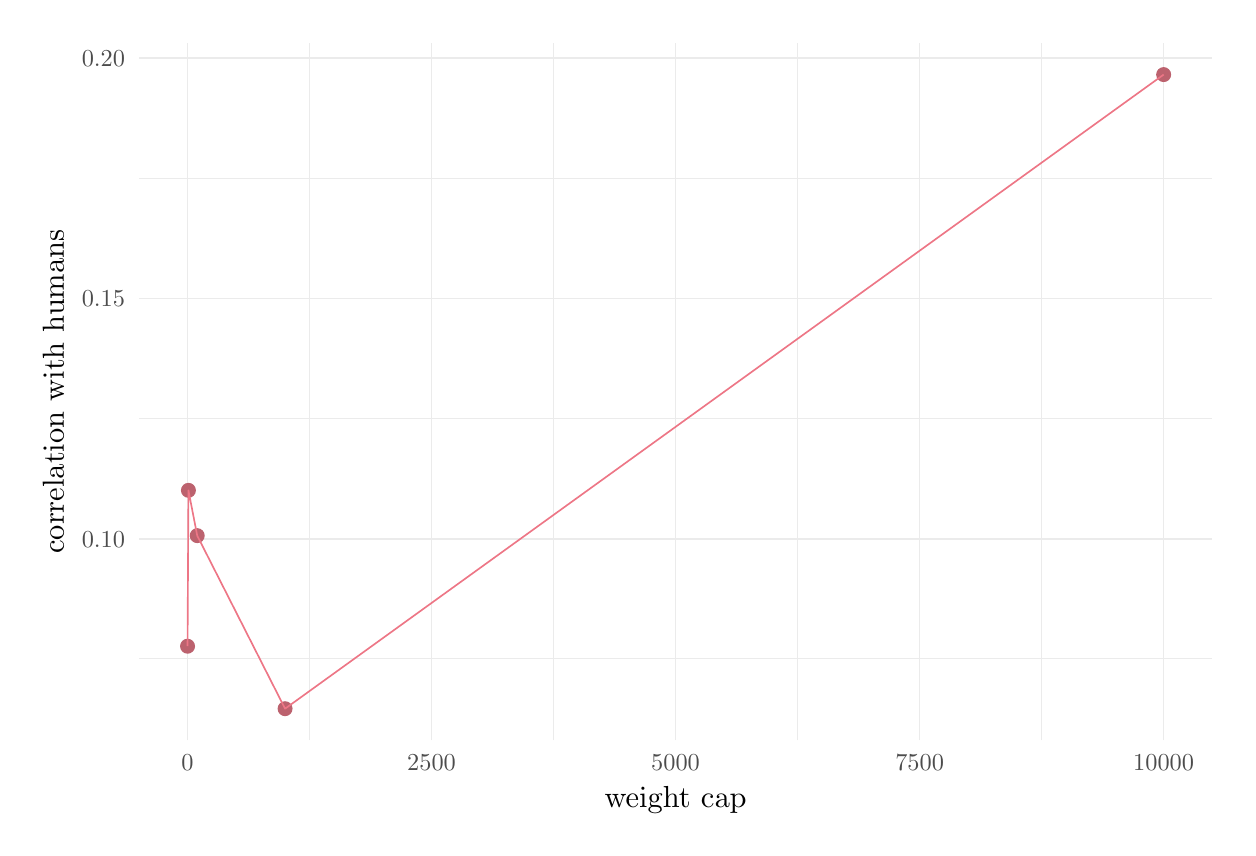
\begin{tikzpicture}[x=1pt,y=1pt]
\definecolor{fillColor}{RGB}{255,255,255}
\path[use as bounding box,fill=fillColor,fill opacity=0.00] (0,0) rectangle (433.62,289.08);
\begin{scope}
\path[clip] ( 40.14, 31.53) rectangle (428.12,283.58);
\definecolor{drawColor}{gray}{0.92}

\path[draw=drawColor,line width= 0.3pt,line join=round] ( 40.14, 60.99) --
	(428.12, 60.99);

\path[draw=drawColor,line width= 0.3pt,line join=round] ( 40.14,147.85) --
	(428.12,147.85);

\path[draw=drawColor,line width= 0.3pt,line join=round] ( 40.14,234.70) --
	(428.12,234.70);

\path[draw=drawColor,line width= 0.3pt,line join=round] (101.83, 31.53) --
	(101.83,283.58);

\path[draw=drawColor,line width= 0.3pt,line join=round] (190.02, 31.53) --
	(190.02,283.58);

\path[draw=drawColor,line width= 0.3pt,line join=round] (278.20, 31.53) --
	(278.20,283.58);

\path[draw=drawColor,line width= 0.3pt,line join=round] (366.39, 31.53) --
	(366.39,283.58);

\path[draw=drawColor,line width= 0.6pt,line join=round] ( 40.14,104.42) --
	(428.12,104.42);

\path[draw=drawColor,line width= 0.6pt,line join=round] ( 40.14,191.27) --
	(428.12,191.27);

\path[draw=drawColor,line width= 0.6pt,line join=round] ( 40.14,278.13) --
	(428.12,278.13);

\path[draw=drawColor,line width= 0.6pt,line join=round] ( 57.74, 31.53) --
	( 57.74,283.58);

\path[draw=drawColor,line width= 0.6pt,line join=round] (145.93, 31.53) --
	(145.93,283.58);

\path[draw=drawColor,line width= 0.6pt,line join=round] (234.11, 31.53) --
	(234.11,283.58);

\path[draw=drawColor,line width= 0.6pt,line join=round] (322.30, 31.53) --
	(322.30,283.58);

\path[draw=drawColor,line width= 0.6pt,line join=round] (410.48, 31.53) --
	(410.48,283.58);
\definecolor{drawColor}{RGB}{188,98,110}
\definecolor{fillColor}{RGB}{188,98,110}

\path[draw=drawColor,line width= 0.4pt,line join=round,line cap=round,fill=fillColor] ( 57.77, 65.57) circle (  2.50);

\path[draw=drawColor,line width= 0.4pt,line join=round,line cap=round,fill=fillColor] ( 58.09,121.89) circle (  2.50);

\path[draw=drawColor,line width= 0.4pt,line join=round,line cap=round,fill=fillColor] ( 61.27,105.52) circle (  2.50);

\path[draw=drawColor,line width= 0.4pt,line join=round,line cap=round,fill=fillColor] ( 93.01, 42.99) circle (  2.50);

\path[draw=drawColor,line width= 0.4pt,line join=round,line cap=round,fill=fillColor] (410.48,272.12) circle (  2.50);
\definecolor{drawColor}{RGB}{237,118,134}

\path[draw=drawColor,line width= 0.6pt,line join=round] ( 57.77, 65.57) --
	( 58.09,121.89) --
	( 61.27,105.52) --
	( 93.01, 42.99) --
	(410.48,272.12);
\end{scope}
\begin{scope}
\path[clip] (  0.00,  0.00) rectangle (433.62,289.08);
\definecolor{drawColor}{gray}{0.30}

\node[text=drawColor,anchor=base east,inner sep=0pt, outer sep=0pt, scale=  0.88] at ( 35.19,101.39) {0.10};

\node[text=drawColor,anchor=base east,inner sep=0pt, outer sep=0pt, scale=  0.88] at ( 35.19,188.24) {0.15};

\node[text=drawColor,anchor=base east,inner sep=0pt, outer sep=0pt, scale=  0.88] at ( 35.19,275.10) {0.20};
\end{scope}
\begin{scope}
\path[clip] (  0.00,  0.00) rectangle (433.62,289.08);
\definecolor{drawColor}{gray}{0.30}

\node[text=drawColor,anchor=base,inner sep=0pt, outer sep=0pt, scale=  0.88] at ( 57.74, 20.52) {0};

\node[text=drawColor,anchor=base,inner sep=0pt, outer sep=0pt, scale=  0.88] at (145.93, 20.52) {2500};

\node[text=drawColor,anchor=base,inner sep=0pt, outer sep=0pt, scale=  0.88] at (234.11, 20.52) {5000};

\node[text=drawColor,anchor=base,inner sep=0pt, outer sep=0pt, scale=  0.88] at (322.30, 20.52) {7500};

\node[text=drawColor,anchor=base,inner sep=0pt, outer sep=0pt, scale=  0.88] at (410.48, 20.52) {10000};
\end{scope}
\begin{scope}
\path[clip] (  0.00,  0.00) rectangle (433.62,289.08);
\definecolor{drawColor}{RGB}{0,0,0}

\node[text=drawColor,anchor=base,inner sep=0pt, outer sep=0pt, scale=  1.10] at (234.13,  7.44) {weight cap};
\end{scope}
\begin{scope}
\path[clip] (  0.00,  0.00) rectangle (433.62,289.08);
\definecolor{drawColor}{RGB}{0,0,0}

\node[text=drawColor,rotate= 90.00,anchor=base,inner sep=0pt, outer sep=0pt, scale=  1.10] at ( 13.08,157.56) {correlation with humans};
\end{scope}
\end{tikzpicture}


}}

\caption{\subref{sfig:scaling_f} Effect of scaling factor for facetted embeddings on the correlation on wordsim353. \subref{sfig:weight_cap} Effect of weight cap for facetted embeddings on the correlation on wordsim353.}
\label{fig:correlation_change}
\end{figure}
\\
\emph{Focal addition and weighing function:} In case of the full similarity using both, focal addition and weighing function, produces the best result. But it is still behind GloVe by a factor of $10$. Word2vec has the best performance on this dataset with the correlation coefficient of $0.52$ .
 \\
 \\
\emph{Adding $1$ to the $log$:} Although adding a $1$ to the $log$ of the weights on its own improves the quality of the model from the basic facetted embedding, combining it with focal addition and a weighing function was proven to be destructive.\\
\\
\emph{Weight cap parameter:} Hyper-parameter of the weighing function to cap the weights ($x_{max}$) plays an important role in the overall performance. $x_{max}=10000$ achieves the best result for this dataset, whereas with the default GloVe model parameters ($100$) performance is reduced. The change of correlation with the weight cap can be seen in the Figure~\ref{sfig:weight_cap}.\\
\\
\emph{Scaling factor parameter:} Same as weight cap, the scaling factor also plays a role in the quality of the model. The same value suggested by the GloVe authors \big($\frac{3}{4}$\big), produced the most promising result. The effect of scaling factor on the correlation is plotted in Figure~\ref{sfig:scaling_f}.\\
\\
\emph{Separate and unified cost functions:} Facetted embedding with the separate and unified cost both achieve the same correlation with human judgment and are considered equal.\\
\\
\emph{Full and partial similarities:} Interestingly, the correlations between the human scores and the facetted method do not change significantly when the dimension is restricted to only the query words. The results can be seen in Figure~\ref{sfig:part_wordsim}, where the correlation between the methods tends to shrink, but the overall score with the humans is more or less stable. From this results, it could be presumed that the most important information about a specific type has been learned through the dimension related to it. 
\\

\begin{figure}
\centering
\subcaptionbox{\label{sfig:full_men}}{
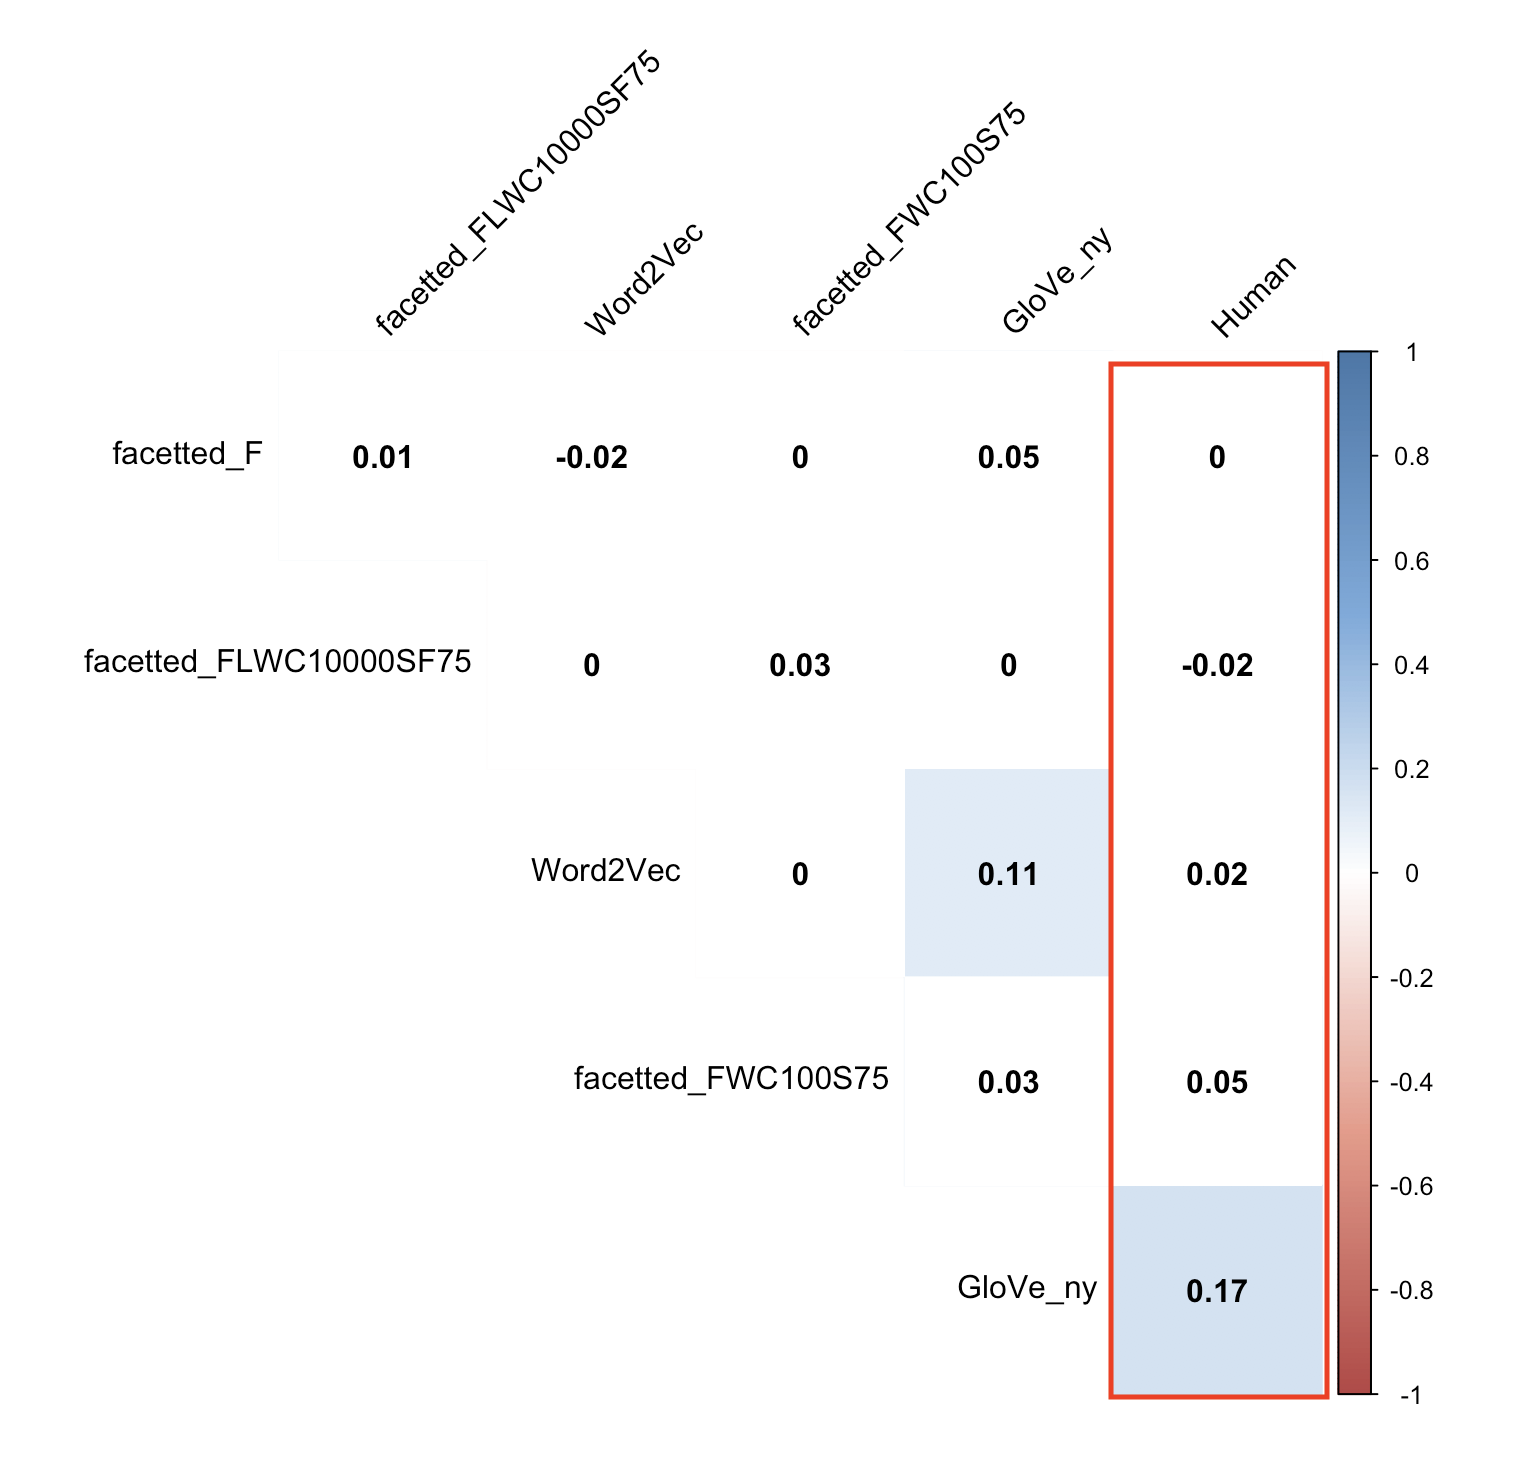
\includegraphics[width=0.7\linewidth , height=0.6\linewidth]{images/men_full.pdf}}
\subcaptionbox{\label{sfig:part_men}}{
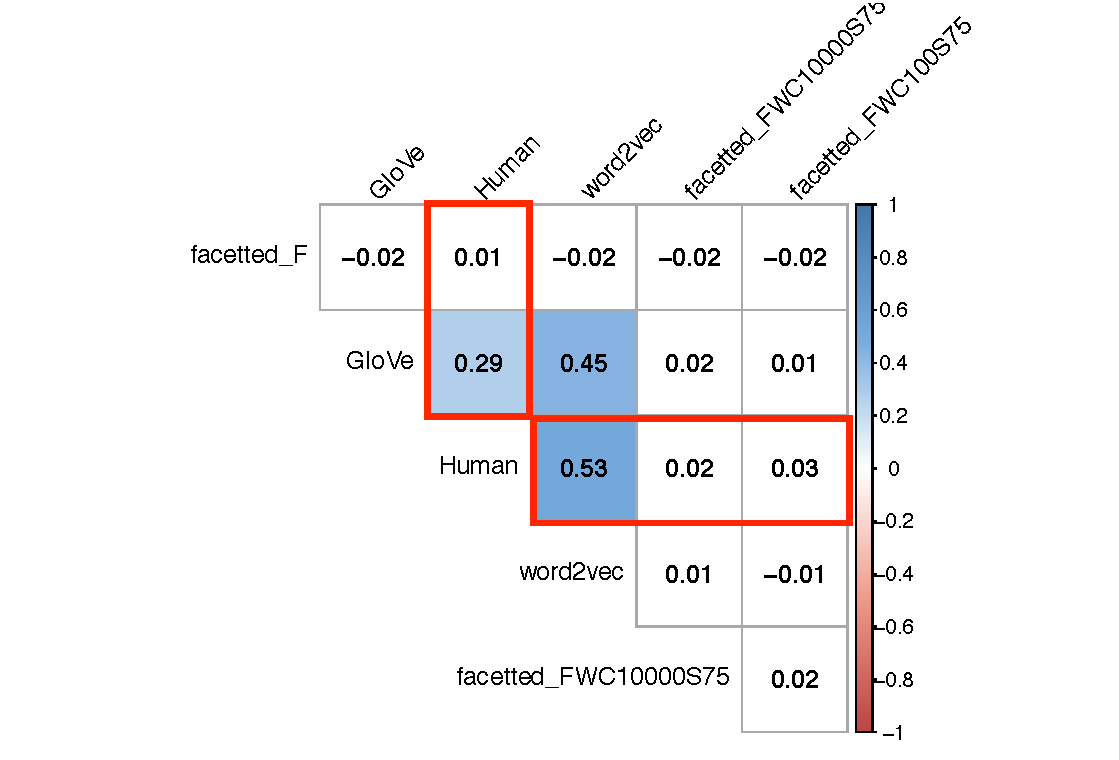
\includegraphics[width=0.7\linewidth , height=0.6\linewidth]{images/men_part.pdf}}

\caption{Correlation plot of the relatedness scores on MEN using the~\subref{sfig:full_men} full vectors and ~\subref{sfig:part_men} using type-specific vectors. Red highlights show the correlation with the human annotations.}
\label{fig:men_cor}
\end{figure}

\noindent
The MEN dataset contains more examples and consequently it is harder to achieve better results. To compare the facetted embedding with GloVe and Word2Vec we only chose the top three models from the previous test, namely:
\begin{itemize}
\item \emph{facetted\_FWC10000S75}, contains focal addition and weighing function with parameters $\alpha=0.75$ and $x_{max}=10000$.
\item  \emph{facetted\_F}, contains only the focal additions.
\item \emph{facetted\_FWC100S75}, contains focal addition and weighing function with parameters $\alpha=0.75$ and $x_{max}=100$.
\end{itemize} 
The results for both full and partial similarities can be seen in Figures~\ref{sfig:full_men} and~\ref{sfig:part_men}. \\
GloVe and word2vec have maintained their performance on the larger dataset, but the correlation with facetted embeddings has decreased dramatically. It can be concluded that there is almost no correlation between annotations in the MEN dataset with facetted embeddings. Changing from full vectors to specific types increased the correlations slightly and even turned \emph{facetted\_FWC10000S75} from a negative to a positive correlation, but not enough to make any noticeable difference.

\begin{figure}
\centering
\subcaptionbox{\label{sfig:word2vec_tsne}}{
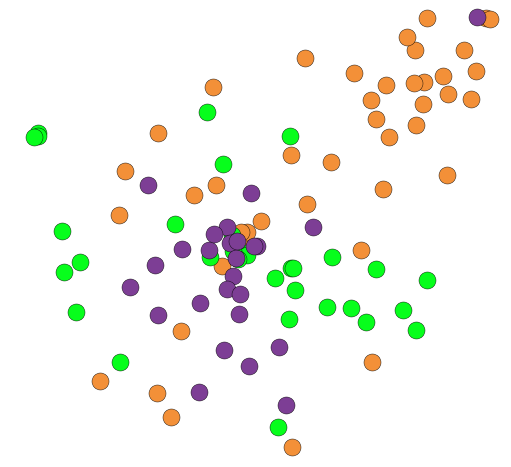
\includegraphics[width=0.48\linewidth , height=0.5\linewidth]{images/tsne_word2vec_cities.png}}
\subcaptionbox{\label{sfig:glove_tsne}}{
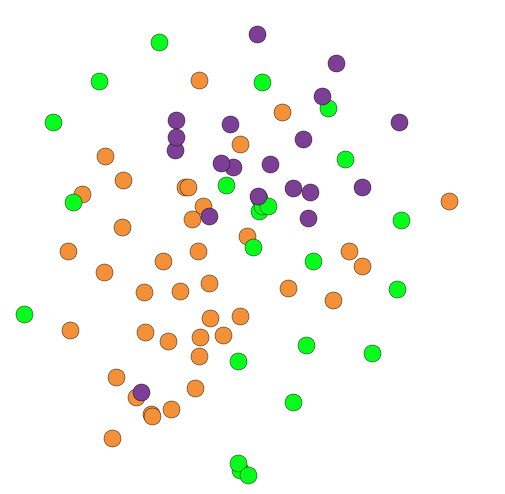
\includegraphics[width=0.48\linewidth , height=0.5\linewidth]{images/tsne_glove_cities.png}}
\subcaptionbox{\label{sfig:complex_tsne}}{
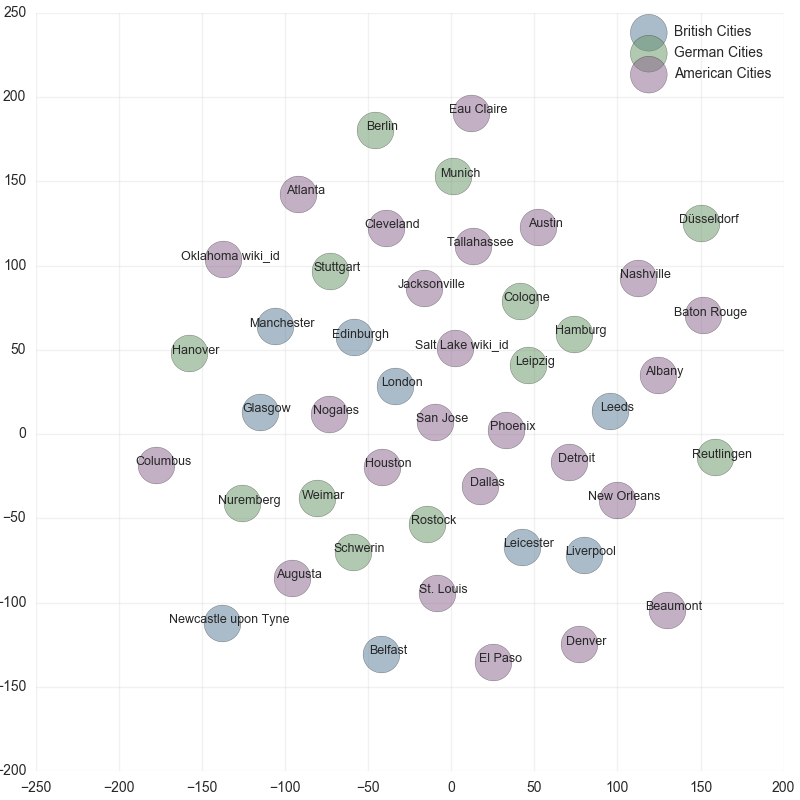
\includegraphics[width=0.5\linewidth , height=0.5\linewidth]{images/tsne_complex_cities.png}}

\caption{t-SNE projections of the embeddings:\subref{sfig:word2vec_tsne} German, British and American cities using Word2Vec \subref{sfig:glove_tsne} GloVe and \subref{sfig:complex_tsne} facetted\_FWC10000S75.}
\label{fig:clust}
\end{figure}




\section{Categorization}\label{sec:categorize}
For clustering similar objects, three test sets were created using \emph{Wikidata Query Service} and were plotted using \emph{t-SNE}. Assuming the embedding dimension can capture the relation to other nearby words well, similar entities would cluster together. The dataset contains:
  \begin{itemize}
    \item ORGanisations of different domains: cars, software companies, websites. 
    \item ACTors of different countries: German politicians, British and American politicians.
    \item LOCations: German, British and American cities.
    \end{itemize}
In each case, up to $30$ entities form each category were chosen based on the highest edge count in LOAD. Some of the results for clustering of LOCations can be seen in Figure~\ref{fig:clust}. In general, no consistent pattern could be found in any of the projections. Although small clusters of objects tend to appear in case of GloVe and our best-selected model for facetted embeddings, most of the entities are scattered without a meaningful cluster. 
\section{Word Analogies}\label{sec:alanlogies}
Many datasets for testing linguistic regularities exist. The most popular one was developed by \cite{DBLP:journals/corr/abs-1301-3781}. The set contains $19,544$ question pairs ($8,869$ semantic and $10,675$ syntactic), with $14$ types of relations ($9$ morphological and $5$ semantic). The types and their meaning are shown in Table~\ref{table:analogy_types}.



\begin{table}[h]
\centering

\begin{tabular}{ll}
        \toprule
{Morphological} & \\         \midrule

gram1-adjective-to-adverb:& an adverb with its adjective.            \\ \hline
gram2-opposite: &noun and its opposite.                          \\ \hline
gram3-comparative: & an adjective with its comparative.                                           \\ \hline
gram4-superlative:&an adjective with its superlative.                                                    \\ \hline
gram5-present-participle:&participles and their verb in infinitive.                                           \\ \hline
gram6-nationality-adjective:&country with its nationality.                                                                \\ \hline
gram7-past-tense: &verbs in infinitive and past form.                                                             \\ \hline
gram8-plural:& nouns in single and plural from.                                                         \\ \hline
gram9-plural-verbs: &verbs in singular and plural.                                                          \\ 
\midrule
\midrule
{Semantic}&\\   
\midrule

capital-common-countries:                 &           selection of countries and their capitals.\\ \hline
capital-world:          &        all countries and their capitals.    \\ \hline
family:     &             family relations such as brother and sister  \\ \hline
city-in-state:   &      states and their cities name (US). \\ \hline
currency:    &        name of a country with its currency.  \\
\bottomrule
\end{tabular}
 \caption{Types of questions in the Mikolovs test, in total $9$
  morphological and $5$ semantic questions.} 
  \label{table:analogy_types}
\end{table}

\begin{table}[h]
  \centering
  {%
    \raisebox{1.5cm}{%
      \begin{tabular}{lSS}
        \toprule
        {Algorithm }                     & {Accuracy}   \\
        \midrule
        Facetted\_FWC10000S75   &0        \\
        GloVe    & 0.008     \\
        word2vec   & 0.015       \\
        \bottomrule
      \end{tabular}
    }
  }
  \caption{The accuracy results on Mikolove's test set with $9,968$ word pairs.}
  \label{table:analogy}
\end{table}

\noindent
After filtering the dataset to match our data we were left with $13$ types (no instance form the  gram6-nationality-adjective set) and $9,968$ word pairs. This test is unbalanced as the number of semantic and morphological relations are not equal. Additionally, \emph{country:capital} relation accounts for over $50$ percent of all semantic questions. As a result, usually, the average accuracy for all semantic/syntactic questions is reported, which has a lot of variations between different parameters, because an embedding might work better in one subcategory, but averaging the mean scores would yield lower results.\\
All the learned embeddings performed poorly on this task. Facetted embeddings were unable to retrieve any of the analogies correctly. GloVe achieved an accuracy of $0.008$ with only $81$ correct pairs and word2vec $0.015$ with $161$ correct pairs. The results can be seen in Table~\ref{table:analogy}. A reason for this behavior could be that our subset does not contain enough tokens to learn many of these relations. On the other hand, most well-known tested models on this dataset are trained on billions of tokens. 
